% Options for packages loaded elsewhere
% Options for packages loaded elsewhere
\PassOptionsToPackage{unicode}{hyperref}
\PassOptionsToPackage{hyphens}{url}
\PassOptionsToPackage{dvipsnames,svgnames,x11names}{xcolor}
%
\documentclass[
  letterpaper,
  DIV=11,
  numbers=noendperiod]{scrartcl}
\usepackage{xcolor}
\usepackage{amsmath,amssymb}
\setcounter{secnumdepth}{5}
\usepackage{iftex}
\ifPDFTeX
  \usepackage[T1]{fontenc}
  \usepackage[utf8]{inputenc}
  \usepackage{textcomp} % provide euro and other symbols
\else % if luatex or xetex
  \usepackage{unicode-math} % this also loads fontspec
  \defaultfontfeatures{Scale=MatchLowercase}
  \defaultfontfeatures[\rmfamily]{Ligatures=TeX,Scale=1}
\fi
\usepackage{lmodern}
\ifPDFTeX\else
  % xetex/luatex font selection
\fi
% Use upquote if available, for straight quotes in verbatim environments
\IfFileExists{upquote.sty}{\usepackage{upquote}}{}
\IfFileExists{microtype.sty}{% use microtype if available
  \usepackage[]{microtype}
  \UseMicrotypeSet[protrusion]{basicmath} % disable protrusion for tt fonts
}{}
\makeatletter
\@ifundefined{KOMAClassName}{% if non-KOMA class
  \IfFileExists{parskip.sty}{%
    \usepackage{parskip}
  }{% else
    \setlength{\parindent}{0pt}
    \setlength{\parskip}{6pt plus 2pt minus 1pt}}
}{% if KOMA class
  \KOMAoptions{parskip=half}}
\makeatother
% Make \paragraph and \subparagraph free-standing
\makeatletter
\ifx\paragraph\undefined\else
  \let\oldparagraph\paragraph
  \renewcommand{\paragraph}{
    \@ifstar
      \xxxParagraphStar
      \xxxParagraphNoStar
  }
  \newcommand{\xxxParagraphStar}[1]{\oldparagraph*{#1}\mbox{}}
  \newcommand{\xxxParagraphNoStar}[1]{\oldparagraph{#1}\mbox{}}
\fi
\ifx\subparagraph\undefined\else
  \let\oldsubparagraph\subparagraph
  \renewcommand{\subparagraph}{
    \@ifstar
      \xxxSubParagraphStar
      \xxxSubParagraphNoStar
  }
  \newcommand{\xxxSubParagraphStar}[1]{\oldsubparagraph*{#1}\mbox{}}
  \newcommand{\xxxSubParagraphNoStar}[1]{\oldsubparagraph{#1}\mbox{}}
\fi
\makeatother


\usepackage{longtable,booktabs,array}
\usepackage{calc} % for calculating minipage widths
% Correct order of tables after \paragraph or \subparagraph
\usepackage{etoolbox}
\makeatletter
\patchcmd\longtable{\par}{\if@noskipsec\mbox{}\fi\par}{}{}
\makeatother
% Allow footnotes in longtable head/foot
\IfFileExists{footnotehyper.sty}{\usepackage{footnotehyper}}{\usepackage{footnote}}
\makesavenoteenv{longtable}
\usepackage{graphicx}
\makeatletter
\newsavebox\pandoc@box
\newcommand*\pandocbounded[1]{% scales image to fit in text height/width
  \sbox\pandoc@box{#1}%
  \Gscale@div\@tempa{\textheight}{\dimexpr\ht\pandoc@box+\dp\pandoc@box\relax}%
  \Gscale@div\@tempb{\linewidth}{\wd\pandoc@box}%
  \ifdim\@tempb\p@<\@tempa\p@\let\@tempa\@tempb\fi% select the smaller of both
  \ifdim\@tempa\p@<\p@\scalebox{\@tempa}{\usebox\pandoc@box}%
  \else\usebox{\pandoc@box}%
  \fi%
}
% Set default figure placement to htbp
\def\fps@figure{htbp}
\makeatother





\setlength{\emergencystretch}{3em} % prevent overfull lines

\providecommand{\tightlist}{%
  \setlength{\itemsep}{0pt}\setlength{\parskip}{0pt}}



 


\KOMAoption{captions}{tableheading}
\makeatletter
\@ifpackageloaded{caption}{}{\usepackage{caption}}
\AtBeginDocument{%
\ifdefined\contentsname
  \renewcommand*\contentsname{Table of contents}
\else
  \newcommand\contentsname{Table of contents}
\fi
\ifdefined\listfigurename
  \renewcommand*\listfigurename{List of Figures}
\else
  \newcommand\listfigurename{List of Figures}
\fi
\ifdefined\listtablename
  \renewcommand*\listtablename{List of Tables}
\else
  \newcommand\listtablename{List of Tables}
\fi
\ifdefined\figurename
  \renewcommand*\figurename{Figure}
\else
  \newcommand\figurename{Figure}
\fi
\ifdefined\tablename
  \renewcommand*\tablename{Table}
\else
  \newcommand\tablename{Table}
\fi
}
\@ifpackageloaded{float}{}{\usepackage{float}}
\floatstyle{ruled}
\@ifundefined{c@chapter}{\newfloat{codelisting}{h}{lop}}{\newfloat{codelisting}{h}{lop}[chapter]}
\floatname{codelisting}{Listing}
\newcommand*\listoflistings{\listof{codelisting}{List of Listings}}
\makeatother
\makeatletter
\makeatother
\makeatletter
\@ifpackageloaded{caption}{}{\usepackage{caption}}
\@ifpackageloaded{subcaption}{}{\usepackage{subcaption}}
\makeatother
\usepackage{bookmark}
\IfFileExists{xurl.sty}{\usepackage{xurl}}{} % add URL line breaks if available
\urlstyle{same}
\hypersetup{
  pdftitle={Clinical Trial On Pleural Cavity Opening During Median Sternotomy},
  pdfauthor={Rafik Margaryan, MD, PhD; Giacomo Bianchi, MD, PhD},
  pdfkeywords={Clinical Trial, Cardiac Surgery},
  colorlinks=true,
  linkcolor={blue},
  filecolor={Maroon},
  citecolor={Blue},
  urlcolor={Blue},
  pdfcreator={LaTeX via pandoc}}


\title{Clinical Trial On Pleural Cavity Opening During Median
Sternotomy}
\author{Rafik Margaryan, MD, PhD \and Giacomo Bianchi, MD, PhD}
\date{2025-04-13}
\begin{document}
\maketitle
\begin{abstract}
Clinicsl Trials are the backbone of the modern medicine. They are the
only way to test securly a hypothesis and to put out an evidence based
medicine. In this paper we will discuss the first and second stage of a
clinical trial on how to make sternotomy without opening plerual
cavities.
\end{abstract}


\section{Introduction}\label{introduction}

The median sternotomy is a common surgical approach used in cardiac
surgery. It provides access to the heart and great vessels, allowing for
various procedures such as coronary artery bypass grafting (CABG), valve
repair or replacement, and aortic surgery. However, one of the potential
complications of median sternotomy is the opening of the pleural
cavities, which can lead to postoperative complications such as
pneumothorax, hemothorax, and respiratory distress.

\section{Data \& Methods}\label{sec-data-methods}

Patients were randomly assigned to two groups: the experimental group,
which underwent median sternotomy with lungs down 10 second and two
thorax compression, and the control group without this maneuver. The
primary outcome was the incidence of pleural cavity opening given two
operators, hospital mortality. Secondary outcomes included length of
hospital stay and postoperative pain from drenages. The data was
collected from a single center and included demographic information,
surgical details, and postoperative outcomes. The data was analyzed
using statistical software to compare the outcomes between the two
groups. \#\# Conclusion

\section{Figures}\label{figures}

\begin{figure}[H]

\centering{

\pandocbounded{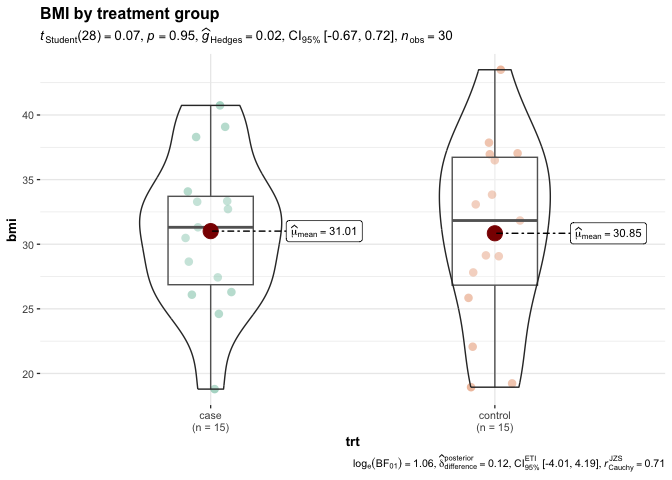
\includegraphics[keepaspectratio]{index_files/figure-latex/notebooks-clinical_trial_first_stage-fig-bmi-first-stage-output-1.png}}

}

\caption{\label{fig-bmi-first-stage}}

\end{figure}%

\textsubscript{Source:
\href{https://raffdoc.github.io/manuscript-template/notebooks/clinical_trial_first_stage-preview.html\#cell-fig-bmi-first-stage}{First
Stage}}

\begin{figure}[H]

\centering{

\pandocbounded{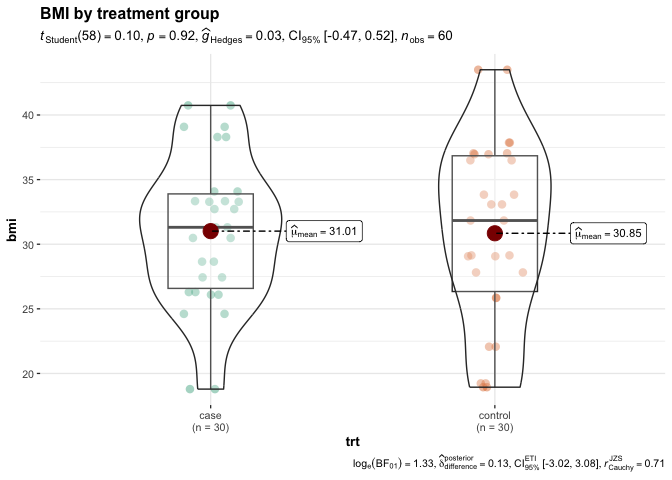
\includegraphics[keepaspectratio]{index_files/figure-latex/notebooks-clinical_trial_second_stage-fig-bmi-second-stage-output-1.png}}

}

\caption{\label{fig-bmi-second-stage}}

\end{figure}%

\textsubscript{Source:
\href{https://raffdoc.github.io/manuscript-template/notebooks/clinical_trial_second_stage-preview.html\#cell-fig-bmi-second-stage}{Second
Stage}}

\section{Tables}\label{tables}

\begin{longtable}[]{@{}
  >{\raggedright\arraybackslash}p{(\linewidth - 2\tabcolsep) * \real{0.4940}}
  >{\raggedright\arraybackslash}p{(\linewidth - 2\tabcolsep) * \real{0.4940}}@{}}

\caption{\label{tbl-demo-stage1}Demographics of the first stage}

\tabularnewline

\toprule\noalign{}
\begin{minipage}[b]{\linewidth}\raggedright
{\textbf{Characteristic}}
\end{minipage} & \begin{minipage}[b]{\linewidth}\raggedright
{\textbf{N = 30}}{\textsuperscript{1}}
\end{minipage} \\
\midrule\noalign{}
\endhead
\bottomrule\noalign{}
\endlastfoot
trt & \begin{minipage}[t]{\linewidth}\raggedright
\hfill\break
\strut
\end{minipage} \\
~~~~case & 15 (50\%) \\
~~~~control & 15 (50\%) \\
outcome & \begin{minipage}[t]{\linewidth}\raggedright
\hfill\break
\strut
\end{minipage} \\
~~~~close & 17 (57\%) \\
~~~~open & 13 (43\%) \\
bmi & 32 (26, 36) \\
diabetis & 12 (40\%) \\
{\textsuperscript{1}} {n (\%); Median (Q1, Q3)} & \\

\end{longtable}

\textsubscript{Source:
\href{https://raffdoc.github.io/manuscript-template/notebooks/clinical_trial_first_stage-preview.html\#cell-tbl-demo-stage1}{First
Stage}}

\begin{longtable}[]{@{}
  >{\raggedright\arraybackslash}p{(\linewidth - 2\tabcolsep) * \real{0.4940}}
  >{\raggedright\arraybackslash}p{(\linewidth - 2\tabcolsep) * \real{0.4940}}@{}}

\caption{\label{tbl-demo-stage2}Demographics of the second stage stage}

\tabularnewline

\toprule\noalign{}
\begin{minipage}[b]{\linewidth}\raggedright
{\textbf{Characteristic}}
\end{minipage} & \begin{minipage}[b]{\linewidth}\raggedright
{\textbf{N = 60}}{\textsuperscript{1}}
\end{minipage} \\
\midrule\noalign{}
\endhead
\bottomrule\noalign{}
\endlastfoot
trt & \begin{minipage}[t]{\linewidth}\raggedright
\hfill\break
\strut
\end{minipage} \\
~~~~case & 30 (50\%) \\
~~~~control & 30 (50\%) \\
outcome & \begin{minipage}[t]{\linewidth}\raggedright
\hfill\break
\strut
\end{minipage} \\
~~~~close & 34 (57\%) \\
~~~~open & 26 (43\%) \\
bmi & 32 (26, 36) \\
diabetis & 24 (40\%) \\
{\textsuperscript{1}} {n (\%); Median (Q1, Q3)} & \\

\end{longtable}

\textsubscript{Source:
\href{https://raffdoc.github.io/manuscript-template/notebooks/clinical_trial_second_stage-preview.html\#cell-tbl-demo-stage2}{Second
Stage}}

\section{Acknowledgements}\label{acknowledgements}

\section*{References}\label{references}
\addcontentsline{toc}{section}{References}

\phantomsection\label{refs}




\end{document}
